% Preamble
\documentclass{beamer}
\usepackage[spanish]{babel}

% Packages
\usepackage{amsmath}
\usepackage[utf8]{inputenc}
\usepackage[T1]{fontenc}
\usepackage{graphicx}
\usepackage{algorithmicx}
\usepackage{algpseudocode}
\usepackage{caption}
\usepackage{courier}

\DeclareMathOperator{\atantwo}{atan2}

\captionsetup{justification=centering, font={scriptsize}, skip=0pt}

% Set bold vectors to satisfy requirements
\renewcommand\vec[1]{\ifstrequal{#1}{0}{\ensuremath{\mathbf{0}}}{\ensuremath{\boldsymbol{#1}}}}

\usetheme[compress]{Berlin}
\usecolortheme{wolverine}
\setbeamertemplate{page number in head/foot}[framenumber]
\setbeamercolor{institute in head/foot}{parent=palette primary}

\title[Dinámica molecular regida por el paso temporal]{Dinámica Molecular regida por el paso temporal}
\subtitle{72.25 - Simulación de Sistemas}
\author[Flores Lucey, Llanos]{Alejo Flores Lucey\inst{1} \and Nehuén Gabriel Llanos\inst{2}}
\institute[Instituto Tecnológico de Buenos Aires]
{
    \inst{1}
    \href{mailto:afloreslucey@itba.edu.ar}{afloreslucey@itba.edu.ar}\\
    Legajo 62622
    \and
    \inst{2}
    \href{mailto:nllanos@itba.edu.ar}{nllanos@itba.edu.ar}\\
    Legajo 62511
}
\date{2024 1C | Grupo Nº3}
\titlegraphic{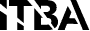
\includegraphics[height=0.5cm]{./itba}}

\makeatletter
\beamer@theme@subsectionfalse
\makeatother

\AtBeginSection[]{
    \begin{frame}
        \begin{beamercolorbox}[sep=8pt,center]{title}
            \usebeamerfont{title}\insertsection
        \end{beamercolorbox}
    \end{frame}
}

\begin{document}

    \begin{frame}
        \titlepage
    \end{frame}

    \section{Oscilador Puntual Amortiguado}

        \begin{frame}{Oscilador Puntual Amortiguado}
            \begin{itemize}
                \item Verlet Original
                \begin{equation*}
                    \begin{cases}
                        r(t + \Delta t) = 2 r(t) - r(t - \Delta t) + \Delta t^2 a(r(t), v(t))\\
                        r(t + \Delta t) = f(r(t), r(t - \Delta t), v(t))
                    \end{cases}
                \end{equation*}
                \begin{equation*}
                      \begin{cases}
                          v(t) = \frac{r(t + \Delta t) - r(t - \Delta t)}{2 \Delta t}\\
                          v(t) = g(r(t + \Delta t), r(t - \Delta t))
                      \end{cases}
                \end{equation*}
                \item Beeman
                \item Gear Predictor-Corrector
                \item Verlet 2.0 (se obtiene $r$ y $v$ para el mismo $\Delta t$.)
                \begin{equation*}
                    \begin{cases}
                        r(t + \Delta t) = f(r(t), r(t - \Delta t), v(t))\\
                        r(t + 2 \Delta t) = f(r(t + \Delta t), r(t), v(t))\\
                        v(t + \Delta t) = g(r(t + 2 \Delta t), r(t))
                    \end{cases}
                \end{equation*}
            \end{itemize}
        \end{frame}

        \begin{frame}{Oscilador Puntual Amortiguado: Resultados}
            \begin{figure}[H!]
                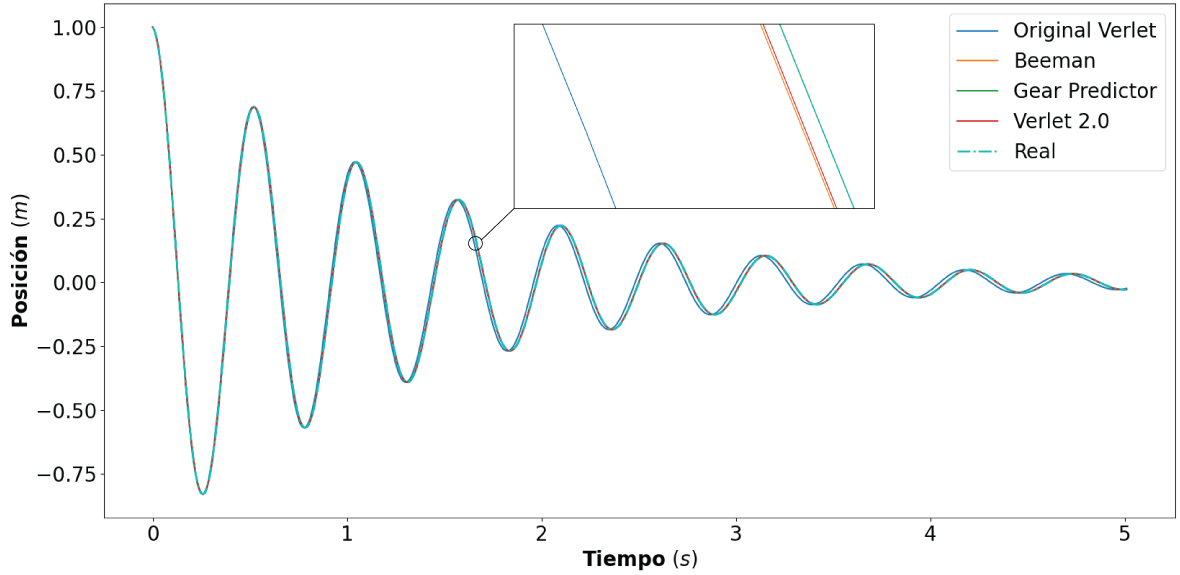
\includegraphics[width=0.9\textwidth]{./oscilador_resultados}
                \label{fig:oscilador_1}
            \end{figure}
        \end{frame}

        \begin{frame}{Oscilador Puntual Amortiguado: Error vs $\Delta t$}
            \begin{figure}[H!]
                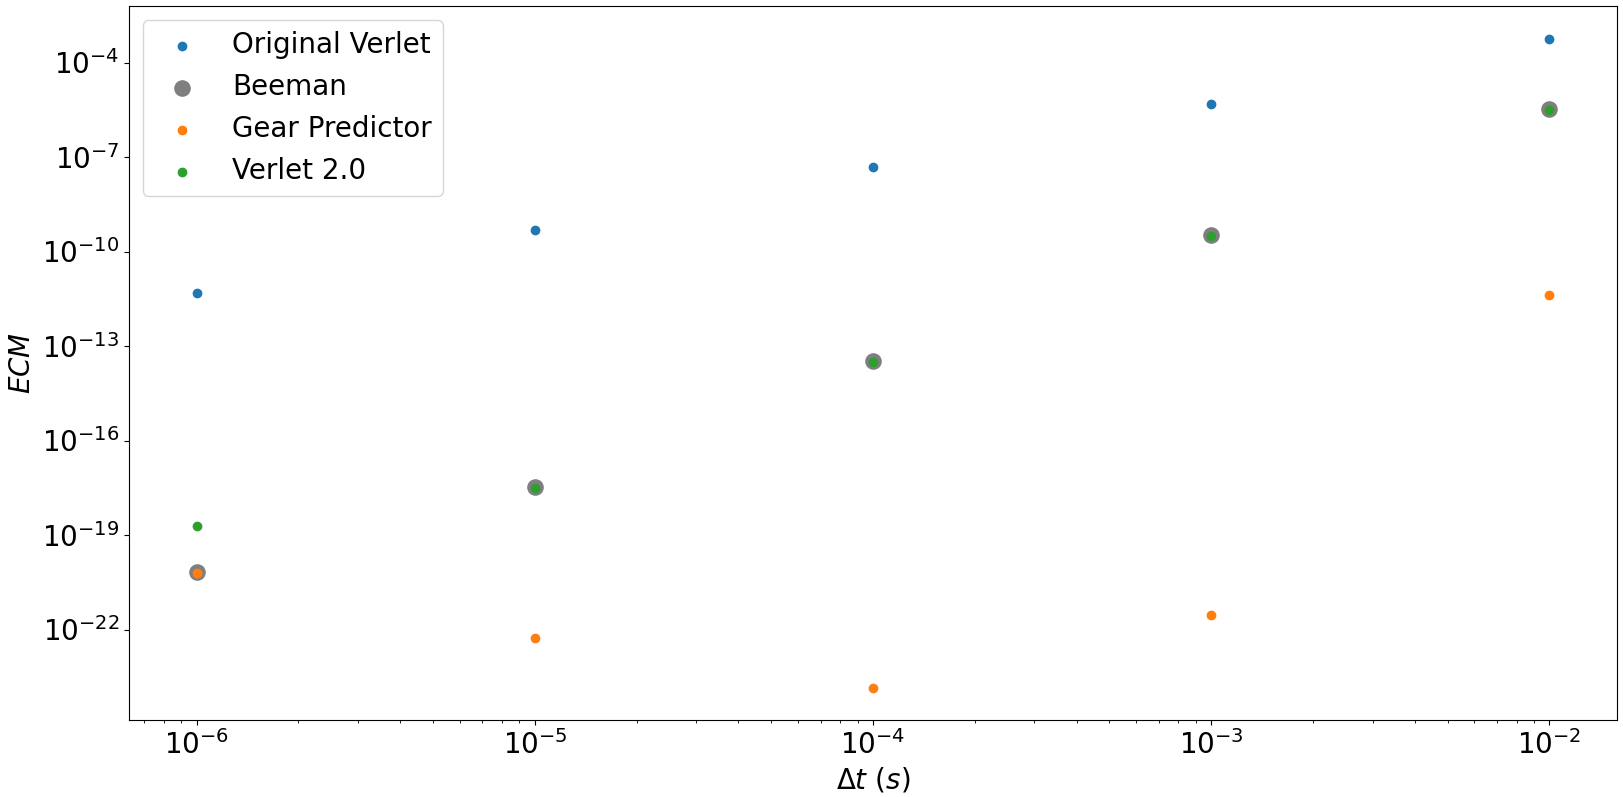
\includegraphics[width=0.9\textwidth]{./oscilador_error}
                \label{fig:oscilador_2}
            \end{figure}
        \end{frame}

    % HASTA ACA ESTÁ CAMBIADO

    \section{Introducción}

        \begin{frame}{Introducción}
            \begin{itemize}
                \item \textbf{Objetivo:}
                \begin{itemize}
                    \item Simular un sistema de partículas en un espacio bidimensional.
                    \item Predecir propiedades de sistemas físicos a nivel de partículas.
                    \item Relacionar observables macroscópicos con dinámicas microscópicas.
                \end{itemize}
                \item \textbf{Modo de simulación:}
                \begin{itemize}
                    \item Simulación dirigida por eventos.
                    \item Se calculan los tiempos de colisión.
                    \item Se avanzan los estados hasta ese tiempo.
                \end{itemize}
            \end{itemize}
        \end{frame}

        \subsection{Sistema Real}

            \begin{frame}{Sistema Real}
                \begin{itemize}
                    \item Las partículas tienen un radio $r$ y una velocidad inicial $\vec{v}$.
                    \item Se estudia como colisionan entre sí y con las paredes del contenedor.
                \end{itemize}
                \begin{minipage}[t]{0.5\textwidth}
                    \begin{itemize}
                        \item \textbf{Aplicaciones:}
                        \begin{itemize}
                            \item Movimiento de moléculas de gas.
                            \item Dinámicas de reacciones químicas.
                            \item Desarrollo de videojuegos.
                        \end{itemize}
                    \end{itemize}
                \end{minipage}
                \hfill
                % HASTA ACA ESTA CAMBIADO
                \begin{minipage}[t]{0.45\textwidth}
                    \begin{figure}[H]
                        \centering
                        \includegraphics[width=\linewidth]{./angrybirds}
                        \label{fig:angry_birds}
                    \end{figure}
                \end{minipage}
            \end{frame}

        \subsection{Fundamentos}

            \begin{frame}{Fundamentos}
                \begin{itemize}
                    \item Las partículas son una 5-upla $(x, y, R, v_x, v_y)$
                    \item Las partículas se mueven en linea recta hasta que ocurre una colisión:
                        \begin{equation*}
                            \vec{x_i}(t+1) = \vec{x_i}(t) + \vec{v_i}(t) t_c\ ; \ t_c = \text{tiempo mínimo de colisión}
                        \end{equation*}
                    \item Se busca el tiempo en el que las partículas colisionan:
                        \begin{equation*}
                            \left( x_i - x_j \right) ^2 + \left( y_i - y_j \right) ^2 = \left( R_i + R_j \right) ^2
                        \end{equation*}
                    \item Las colisiones son elásticas y se conserva el impulso.
                \end{itemize}
            \end{frame}

    \section{Implementación}

        \subsection{Arquitectura}

            \begin{frame}{Diagrama UML}
                \begin{figure}[htbp]
                    \centering
                    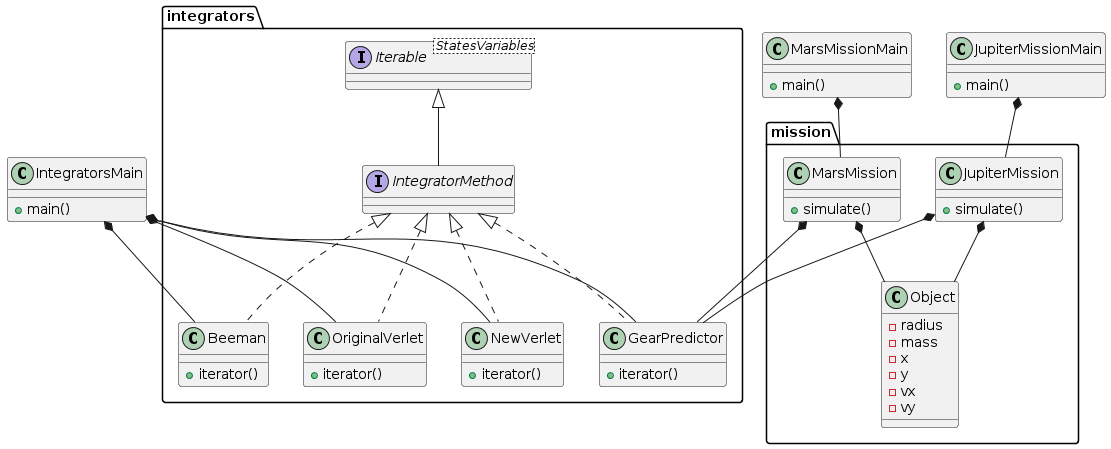
\includegraphics[width=\textwidth]{./architecture}
                    \label{fig:architecture}
                \end{figure}
            \end{frame}

        \subsection{Algoritmo}

            \begin{frame}{Pseudocódigo del algoritmo implementado}{}
                \begin{algorithmic}[1]
                    \ttfamily \scriptsize
                    \State Create output file
                    \State collisions $\gets$ new OrderedSet()
                    \ForAll{p $\in$ particles}
                        \State collisions $\gets$ \Call{CalculateCollisionsWithWalls}{p}
                        \ForAll{q $\in$ particles}
                            \State collisions $\gets$ \Call{CalculateCollisionsBetweenParticles}{p, q}
                        \EndFor
                    \EndFor
                    \While{$i < eventCount$}
                        \State first $\gets$ \Call{PopFirstCollision}{collisions}
                        \ForAll{p $\in$ particles}
                            \State \Call{Move}{p, first.time}
                        \EndFor
                        \State \Call{UpdateCollisionsTime}{first.time}
                        \State \Call{WriteOutput}{particles}
                        \State \Call{UpdateVelocities}{first.p1, first.p2}
                        \State \Call{CalculateNewCollisions}{first}
                        \State $i \gets i + 1$
                    \EndWhile
                \end{algorithmic}
            \end{frame}

    \section{Simulaciones}

        \subsection{Parámetros de entrada}

            \begin{frame}{Parámetros de entrada}
                \begin{itemize}
                    \item Parámetros de entrada fijos:
                    \begin{itemize}
                        \item Número de partículas ($N$): \alert{$300$}
                        \item Cantidad de eventos ($E$): \alert{$20\,000$}
                        \item Longitud del plano ($L$): \alert{$0.1 m$}
                        \item Radio de partículas ($r$): \alert{$0.001 m$}
                        \item Radio del obstáculo ($R$): \alert{$0.005 m$}
                        \item Masa de partículas ($m$): \alert{$1 kg$}
                        \item Masa del obstáculo ($m$): \alert{$3 kg$}
                    \end{itemize}
                    \item Parámetros de entrada variables:
                    \begin{itemize}
                        \item Módulo de la velocidad inicial ($v_0$): \alert{$\{1, 3, 6, 10\} m/s$}
                    \end{itemize}
                \end{itemize}
            \end{frame}

        \subsection{Observables}

            \begin{frame}{Presión en paredes y obstáculo en función del tiempo ($P(t)$)}
                \begin{itemize}
                    \item Presión en paredes en función del tiempo:
                    \begin{equation*}
                        P_{Paredes}(t) = \frac{\sum \Delta V_{n\ (Paredes)}}{\Delta t \cdot L \cdot 4}
                    \end{equation*}
                    \begin{equation*}
                        v_{n\ (Paredes\ Sup.\ y\ Inf.)} = \left| v \cdot \sin(\alpha) \cdot 2 \right|
                    \end{equation*}
                    \begin{equation*}
                        v_{n\ (Paredes\ Izq.\ y\ Der.)} = \left| v \cdot \cos(\alpha) \cdot 2 \right|
                    \end{equation*}
                    \item Presión en el obstáculo en función del tiempo:
                    \begin{equation*}
                        P_{Obst\acute{a}culo}(t) = \frac{\sum \vec{v_{n\ (Obst\acute{a}culo)}}}{\Delta t \cdot 2\pi \cdot R}
                    \end{equation*}
                    \begin{equation*}
                          \vec{v_{n\ (Obst\acute{a}culo)}} = \left| {v \cdot \cos \left( \atantwo \left(\frac{L}{2} - y, \frac{L}{2} - x \right) \right) \cdot 2} \right|
                    \end{equation*}
                \end{itemize}
            \end{frame}

            \begin{frame}{Tiempo en el que el nro. de choques alcanza el 20\% de $N$ }
                \begin{itemize}
                    \item Se realizan diez (10) corridas.
                    \item Se estudia el tiempo en el que el 20\% de las partículas colisionan por primera vez con el obstáculo.
                    \begin{equation*}
                        t_{\text{prom}} = \frac{\sum_{i=1}^{10} t_i}{10} \ ,\ t_i\text{: tiempo en corrida }i
                    \end{equation*}
                    \begin{equation*}
                        \sigma = \sqrt{\frac{1}{9} \sum_{i=1}^{10} (t_i - t_{\text{prom}})^2}
                    \end{equation*}
                \end{itemize}
            \end{frame}

            \begin{frame}{Número de choques por unidad de tiempo}
                \begin{itemize}
                    \item Se calcula la pendiente de la curva mediante el método de regresión lineal simple
                    \begin{equation*}
                        \begin{split}
                            m_k(\iota) = \frac{\iota \sum_{i=1}^\iota x_i y_i - \sum_{i=1}^\iota x_i \sum_{i=1}^\iota y_i }{\iota \sum_{i=1}^\iota x_i^2 - \left(\sum_{i=1}^\iota x_i \right)^2}
                            \ , 1 \leq k \leq 10
                            \\ \iota = \text{cantidad de choques en el intervalo de tiempo}
                        \end{split}
                    \end{equation*}
                    \item Se promedian los valores obtenidos de cada una de las diez (10) corridas y se calcula su error asociado:
                    \begin{equation*}
                            m_{prom} = \frac{1}{10} \sum_{i=1}^{10} m_i
                        \text{ ; }
                            \sigma = \sqrt{\frac{1}{9} \sum_{i=1}^{10} (m_i - m_{\text{prom}})^2}
                    \end{equation*}
                \end{itemize}
            \end{frame}

            \begin{frame}{Desplazamiento cuadrático medio ($DCM$)}
                \begin{itemize}
                    \item Se realiza para cuatro (4) velocidades y diez (10) corridas cada una.
                    \item Se divide el intervalo de tiempo en cien (100) $\Delta t$.
                    \item Se obtiene el desplazamiento cuadrático medio para cada $\Delta t$:
                    \begin{equation*}
                        DCM_{\Delta t} = \frac{\sum_{i=1}^{10} \left( x_{t_i} - x_0 \right)^2 + \left( y_{t_i} - y_0 \right)^2}{10}
                    \end{equation*}
                \end{itemize}
            \end{frame}

            \begin{frame}{Coeficiente de difusión ($D$)}
                \begin{itemize}
                    \item Se obtiene la pendiente de la curva de $DCM$ en función del tiempo mediante el método
                    de regresión lineal simple para cada velocidad.
                    \begin{equation*}
                        m_v = \frac{100 \sum_{i=1}^{100} x_i y_i - \sum_{i=1}^{100} x_i \sum_{i=1}^{100} y_i }{100 \sum_{i=1}^{100} x_i^2
                        - \left(\sum_{i=1}^{100} x_i \right)^2},\ v \in \{1, 3, 6, 10\}
                    \end{equation*}
                    \item Se obtiene el coeficiente de difusión:
                    \begin{equation*}
                        D_v = \frac{m_v}{4},\ v \in \{1, 3, 6, 10\}
                    \end{equation*}
                \end{itemize}
            \end{frame}

    \section{Resultados}

        \subsection{Animación del sistema}

            \begin{frame}{Sistema con $v_0=1m/s$}{Animación}
                \begin{minipage}[t]{0.60\textwidth}
                    \begin{figure}[H!]
                        \includegraphics[height=.65\textheight]{./animation_obstacle_still_v_1}
                        \caption*{Véase la animación completa en \url{https://youtu.be/6y7aywkQ5ro}.}
                        \label{fig:a_1}
                    \end{figure}
                \end{minipage}
                \hfill
                \begin{minipage}[t]{0.30\textwidth}
                    \begin{block}{Datos del sistema}
                        \begin{itemize}
                            \item $N=300$
                            \item $E=20\,000$
                            \item $v_0 = 1 m/s$
                        \end{itemize}
                    \end{block}
                \end{minipage}
            \end{frame}

            \begin{frame}{Sistema con $v_0 \in \{ 3, 6, 10\}m/s$}{Animación}
                \begin{minipage}[t]{0.3\textwidth}
                    \begin{figure}[H!]
                        \includegraphics[width=\textwidth]{./animation_obstacle_still_v_3}
                        \caption*{Véase la animación completa en \url{https://youtu.be/e0YvqmfTLc4}.}
                        \label{fig:a_2}
                    \end{figure}
                    \begin{beamercolorbox}[sep=5pt,center]{block body}
                        \centering
                        \small{$v_0=3m/s$}
                    \end{beamercolorbox}
                \end{minipage}
                \hfill
                \begin{minipage}[t]{0.30\textwidth}
                    \begin{figure}[H!]
                        \includegraphics[width=\textwidth]{./animation_obstacle_still_v_6}
                        \caption*{Véase la animación completa en \url{https://youtu.be/DVVqFmP-cuQ}.}
                        \label{fig:a_3}
                    \end{figure}
                    \begin{beamercolorbox}[sep=5pt,center]{block body}
                        \centering
                        \small{$v_0=6m/s$}
                    \end{beamercolorbox}
                \end{minipage}
                \hfill
                \begin{minipage}[t]{0.30\textwidth}
                    \begin{figure}[H!]
                        \includegraphics[width=\textwidth]{./animation_obstacle_still_v_10}
                        \caption*{Véase la animación completa en \url{https://youtu.be/8M5MV5kRghI}.}
                        \label{fig:a_4}
                    \end{figure}
                    \begin{beamercolorbox}[sep=5pt,center]{block body}
                        \centering
                        \small{$v_0=10m/s$}
                    \end{beamercolorbox}
                \end{minipage}
            \end{frame}

        \subsection{Presión en paredes y obstáculo}

            \begin{frame}{Presión vs Tiempo con $v_0=1m/s$}{Observable: Presión}
                    \begin{figure}[H!]
                        \includegraphics[width=0.9\textwidth]{./pressure_vs_time_1}
                        \label{fig:p_1}
                    \end{figure}
                    \begin{beamercolorbox}[sep=5pt,center]{block body}
                        \begin{minipage}[t]{0.3\textwidth}
                            \centering
                            \small{$N=300$}
                        \end{minipage}
                        \hfill
                        \begin{minipage}[t]{0.3\textwidth}
                            \centering
                            \small{$E=20\,000$}
                        \end{minipage}
                        \hfill
                        \begin{minipage}[t]{0.3\textwidth}
                            \centering
                            \small{$v_0 = 1 m/s$}
                        \end{minipage}
                    \end{beamercolorbox}
            \end{frame}

            \begin{frame}{Presión vs Temperatura}{Observable: Presión}
                \begin{figure}[H!]
                    \includegraphics[width=0.9\textwidth]{./pressure_vs_temperature}
                    \label{fig:p_vs_t}
                \end{figure}
                \begin{beamercolorbox}[sep=5pt,center]{block body}
                    \begin{minipage}[t]{0.3\textwidth}
                        \centering
                        \small{$N=300$}
                    \end{minipage}
                    \hfill
                    \begin{minipage}[t]{0.3\textwidth}
                        \centering
                        \small{$E=20\,000$}
                    \end{minipage}
                \end{beamercolorbox}
            \end{frame}

        \subsection{Tiempo en el que el 20\% de las partículas colisionan con el obstáculo}

            \begin{frame}{Número de Colisiones vs Tiempo}{Observable: Tiempo en el que el 20\% de las partículas colisionan con el obstáculo}
                \begin{figure}[H!]
                    \includegraphics[width=0.9\textwidth]{./unique_collisions_vs_time}
                    \label{fig:threshold_1}
                \end{figure}
                \begin{beamercolorbox}[sep=5pt,center]{block body}
                    \begin{minipage}[t]{0.45\textwidth}
                        \centering
                        \small{$N=300$}
                    \end{minipage}
                    \hfill
                    \begin{minipage}[t]{0.45\textwidth}
                        \centering
                        \small{$E=20\,000$}
                    \end{minipage}
                \end{beamercolorbox}
            \end{frame}

            \begin{frame}{Observable vs Temperatura}{Observable: Tiempo en el que el 20\% de las partículas colisionan con el obstáculo}
                \begin{figure}[H!]
                    \includegraphics[width=0.9\textwidth]{./threshold_vs_temperature}
                    \label{fig:threshold_2}
                \end{figure}
                \begin{beamercolorbox}[sep=5pt,center]{block body}
                    \begin{minipage}[t]{0.45\textwidth}
                        \centering
                        \small{$N=300$}
                    \end{minipage}
                    \hfill
                    \begin{minipage}[t]{0.45\textwidth}
                        \centering
                        \small{$E=20\,000$}
                    \end{minipage}
                \end{beamercolorbox}
            \end{frame}

        \subsection{Nro. de colisiones con el obstáculo por unidad de tiempo}

            \begin{frame}{Número de Colisiones vs Tiempo}{Observable: Nro. de colisiones con el obstáculo por unidad de tiempo}
                \begin{figure}[H!]
                    \includegraphics[width=0.9\textwidth]{./total_collisions_vs_time}
                    \label{fig:slope_1}
                \end{figure}
                \begin{beamercolorbox}[sep=5pt,center]{block body}
                    \begin{minipage}[t]{0.45\textwidth}
                        \centering
                        \small{$N=300$}
                    \end{minipage}
                    \hfill
                    \begin{minipage}[t]{0.45\textwidth}
                        \centering
                        \small{$E=20\,000$}
                    \end{minipage}
                \end{beamercolorbox}
            \end{frame}

            \begin{frame}{Observable vs Temperatura}{Observable: Nro. de colisiones con el obstáculo por unidad de tiempo}
                \begin{figure}[H!]
                    \includegraphics[width=0.9\textwidth]{./slope_vs_temperature}
                    \label{fig:slope_2}
                \end{figure}
                \begin{beamercolorbox}[sep=5pt,center]{block body}
                    \begin{minipage}[t]{0.45\textwidth}
                        \centering
                        \small{$N=300$}
                    \end{minipage}
                    \hfill
                    \begin{minipage}[t]{0.45\textwidth}
                        \centering
                        \small{$E=20\,000$}
                    \end{minipage}
                \end{beamercolorbox}
            \end{frame}

        \subsection{Desplazamiento Cuadrático Medio}

            \begin{frame}{Sistema con $v_0=1m/s$ y obstáculo en movimiento}{Animación}
                \begin{minipage}[t]{0.60\textwidth}
                    \begin{figure}[H!]
                        \includegraphics[height=.65\textheight]{./animation_obstacle_moves_v_1}
                        \caption*{Véase la animación completa en \url{https://youtu.be/ZB0ikr5PKak}.}
                        \label{fig:a_5}
                    \end{figure}
                \end{minipage}
                \hfill
                \begin{minipage}[t]{0.30\textwidth}
                    \begin{block}{Datos del sistema}
                        \begin{itemize}
                            \item $N=300$
                            \item $E=20\,000$
                            \item Partículas:
                            \begin{itemize}
                                \item $m = 1 kg$
                                \item $v_0 = 1 m/s$
                            \end{itemize}
                            \item Obstáculo:
                            \begin{itemize}
                                \item $m = 3 kg$
                                \item $v_0 = 0 m/s$
                            \end{itemize}
                        \end{itemize}
                    \end{block}
                \end{minipage}
            \end{frame}

            \begin{frame}{Desplazamiento Cuadrático vs Tiempo}{Observable: Desplazamiento Cuadrático Medio}
                \begin{figure}[H!]
                    \includegraphics[width=0.9\textwidth]{./dc_vs_time_1}
                    \label{fig:dcm_1}
                \end{figure}
                \begin{beamercolorbox}[sep=5pt,center]{block body}
                    \begin{minipage}[t]{0.24\textwidth}
                        \centering
                        \small{$N=300$}
                    \end{minipage}
                    \hfill
                    \begin{minipage}[t]{0.24\textwidth}
                        \centering
                        \small{$E=20\,000$}
                    \end{minipage}
                    \hfill
                    \begin{minipage}[t]{0.24\textwidth}
                        \centering
                        \small{$v_0 = 1 m/s$}
                    \end{minipage}
                    \hfill
                    \begin{minipage}[t]{0.24\textwidth}
                        \centering
                        \small{$\#Corridas = 10$}
                    \end{minipage}
                \end{beamercolorbox}
            \end{frame}

            \begin{frame}{Desplazamiento Cuadrático Medio vs Tiempo}{Observable: Desplazamiento Cuadrático Medio}
                \begin{figure}[H!]
                    \includegraphics[width=0.9\textwidth]{./dcm_vs_time}
                    \label{fig:dcm_2}
                \end{figure}
                \begin{beamercolorbox}[sep=5pt,center]{block body}
                    \begin{minipage}[t]{0.3\textwidth}
                        \centering
                        \small{$N=300$}
                    \end{minipage}
                    \hfill
                    \begin{minipage}[t]{0.3\textwidth}
                        \centering
                        \small{$E=20\,000$}
                    \end{minipage}
                    \hfill
                    \begin{minipage}[t]{0.3\textwidth}
                        \centering
                        \small{$\#Corridas = 10$}
                    \end{minipage}
                \end{beamercolorbox}
            \end{frame}

            \begin{frame}{Coeficiente de Difusión vs Temperatura}{Observable: Coeficiente de Difusión}
                \begin{figure}[H!]
                    \includegraphics[width=0.9\textwidth]{./coefficient_diffusion_vs_temperature}
                    \label{fig:dcm_3}
                \end{figure}
                \begin{beamercolorbox}[sep=5pt,center]{block body}
                    \begin{minipage}[t]{0.3\textwidth}
                        \centering
                        \small{$N=300$}
                    \end{minipage}
                    \hfill
                    \begin{minipage}[t]{0.3\textwidth}
                        \centering
                        \small{$E=20\,000$}
                    \end{minipage}
                    \hfill
                    \begin{minipage}[t]{0.3\textwidth}
                        \centering
                        \small{$\#Corridas = 10$}
                    \end{minipage}
                \end{beamercolorbox}
            \end{frame}

    \section{Conclusiones}

        \begin{frame}{Conclusiones}
            \begin{block}{Presión del sistema}
                \begin{itemize}
                    \item Aumenta linealmente con la temperatura.
                    \item \textbf{Se comporta como un gas ideal.}
                    \item Se mantiene constante en el tiempo.
                    \item La presión en el obstáculo es igual que en las paredes.
                \end{itemize}
            \end{block}
            \begin{block}{Tiempo en el que el 20\% de las partículas colisionan con el obstáculo}
                \begin{itemize}
                    \item Disminuye exponencialmente con la temperatura.
                    \item Se debe a la mayor energía cinética de las partículas.
                \end{itemize}
            \end{block}
        \end{frame}

        \begin{frame}{Conclusiones}
            \begin{block}{Número de colisiones con el obstáculo por unidad de tiempo}
                \begin{itemize}
                    \item Aumenta logarítmicamente con la temperatura.
                \end{itemize}
            \end{block}
            \begin{block}{Desplazamiento Cuadrático Medio}
                \begin{itemize}
                    \item Se llega más rápido al estacionario con mayor temperatura.
                    \item El coeficiente de difusión aumenta con la temperatura.
                    \item El coeficiente de difusión alcanza un valor estacionario.
                    \item \textbf{Se comporta como los elementos de la naturaleza.}
                \end{itemize}
            \end{block}
        \end{frame}

        \begin{frame}
            \begin{beamercolorbox}[sep=8pt,center]{title}
                \usebeamerfont{title}{¡Muchas gracias!}
            \end{beamercolorbox}
        \end{frame}

\end{document}
